% Provenance (never printed): see sources/outline_sources.md (Year 3: the
% structure of the Galaxy; the rotation curve and dark matter; galaxy types;
% the distance ladder, Hubble's law recalled from the physics books).
% Brief: sources/book5/BRIEFS.md, ch. 29. Curves from figdata/bachelor-3/
% rotation_curve.py (the circular velocity curve of Eilers et al. 2019 with the
% Pouliasis et al. 2017 Model I baryons and an NFW halo fitted to it) and
% distance_ladder.py (the OGLE-IV Cepheids of the Large Magellanic Cloud, CDS
% J/AcA/65/297, and the ranges of the rungs). Exercise and problem values in the
% Book 5 scratch calculator calc/ch29.py. The survey of Part I of the problem and
% the galaxies of the exercises are invented.
\chapter{La Vía Láctea y las galaxias}\label{ch:b3:milky-way-galaxies}

En el Sistema Solar, los planetas alejados del Sol se mueven lentamente: Mercurio
lo recorre a \qty{47.4}{km.s^{-1}}, Neptuno a \qty{5.4}{km.s^{-1}}, como
exige la tercera ley de Kepler a los cuerpos ligados a una única masa central. Las estrellas
de la Galaxia no se comportan así. Medida a partir de los movimientos de más de
veinte mil gigantes rojas, la velocidad de sus órbitas circulares es
\qty{227}{km.s^{-1}} a \qty{5}{kpc} del centro, \qty{229}{km.s^{-1}}
en el Sol, y todavía \qty{198}{km.s^{-1}} a \qty{25}{kpc}, donde apenas
quedan estrellas ni gas. Si la masa que vemos fuera toda la que existe, las estrellas
exteriores se moverían mucho más despacio. Algo no visible las retiene. Este capítulo
describe la Galaxia en la que vivimos, la pesa a partir de su rotación, clasifica las
demás galaxias por tipos y recorre la cadena de métodos con los que se miden sus
distancias y la expansión del Universo.
% ledger: planet:Mercury.vorb, planet:Neptune.vorb, eilers19:vc, eilers19:table1

\begin{recall}
La Vía Láctea, el efecto Doppler, las leyes de Kepler, el teorema de Newton sobre la
atracción de una capa esférica, la materia oscura, los agujeros negros y su
radio de Schwarzschild, las supernovas, las enanas blancas, la línea de 21 cm del
hidrógeno atómico y la ley de Hubble se estudian en los libros de física. El paralaje anual,
el parsec, el flujo y la luminosidad, las magnitudes aparente y absoluta, el
módulo de distancia, las bandas fotométricas y el índice de color están en el
volumen de primer año, en su capítulo sobre telescopios y fotometría. El
medio interestelar y su polvo están en el volumen de segundo año, en su capítulo
sobre el medio interestelar y la formación estelar.
\end{recall}

\section{La estructura de la Galaxia}\label{sec:b3:milky-way-galaxies:structure}

Vista desde la Tierra, la Galaxia es la Vía Láctea: una banda de luz que rodea
todo el cielo, atravesada por oscuras franjas de polvo y más brillante hacia la
constelación de Sagitario, donde se encuentra su centro. La banda es el disco en
el que se halla el Sol, visto de canto desde dentro.

\begin{omfigure}
\centering
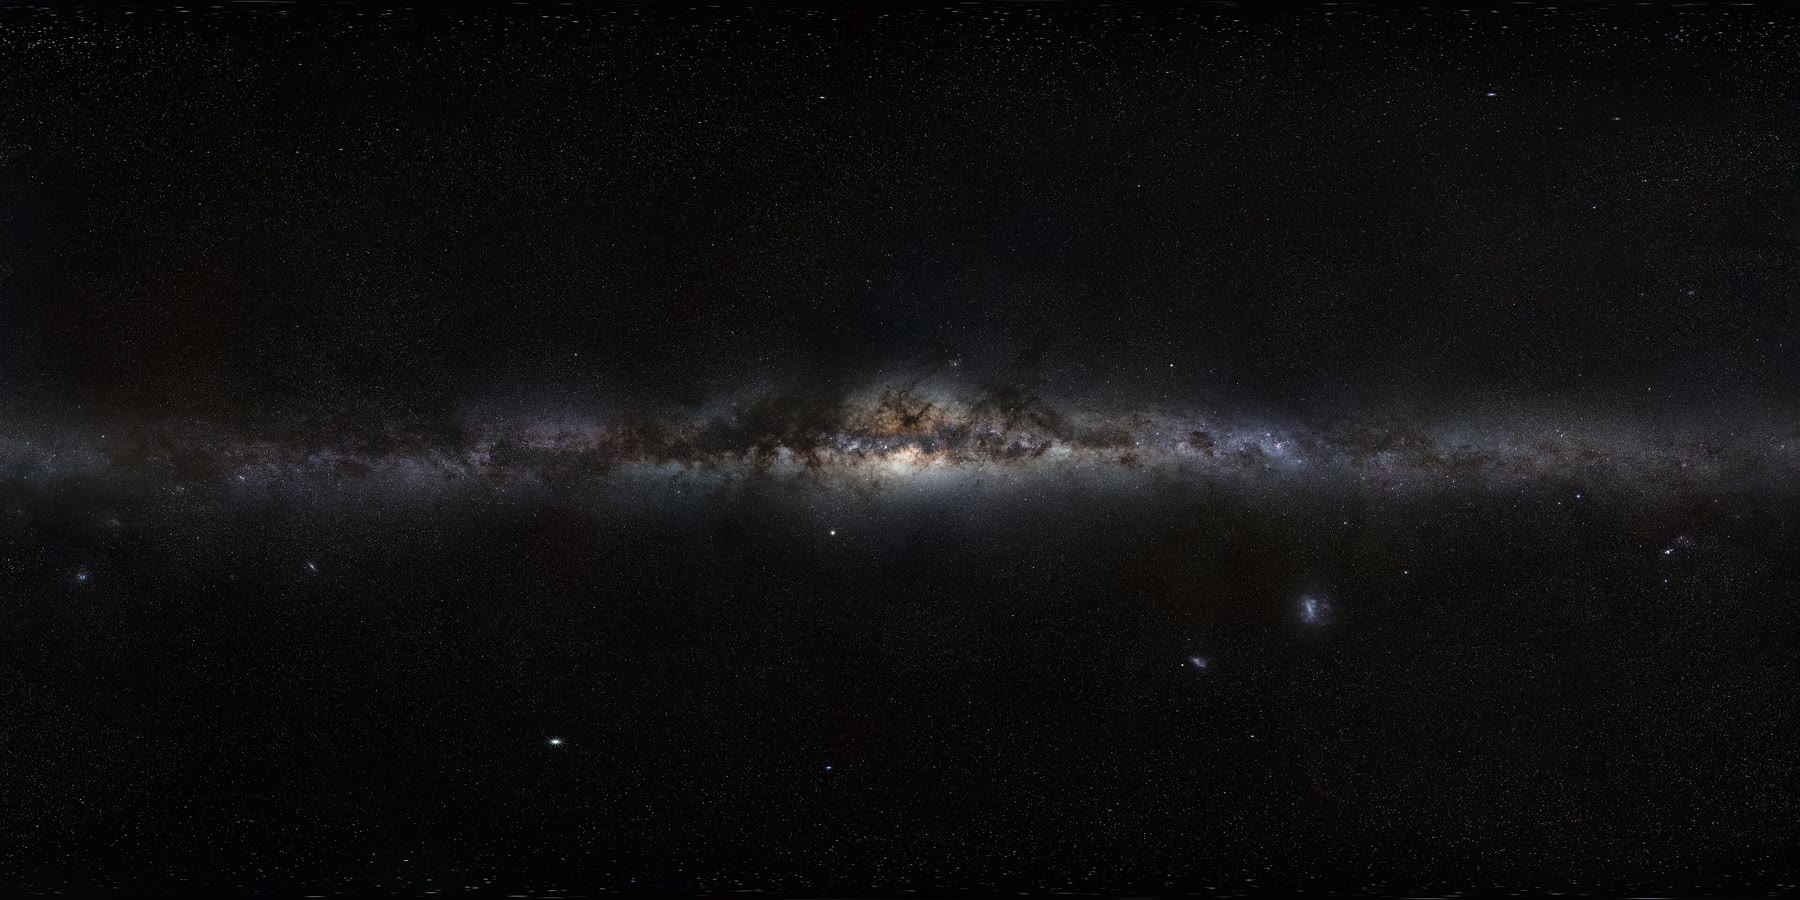
\includegraphics[width=0.96\linewidth]{images/book5/b3-milky-way-panorama.jpg}
\par\smallskip{\small Todo el cielo en una sola imagen, proyectado de modo que el
plano de la Galaxia atraviesa el centro y su núcleo queda en el
centro de la imagen. La banda es el disco visto desde dentro; las oscuras
franjas son polvo del disco, que oculta las estrellas situadas detrás; el bulbo central
se abulta alrededor del centro. Las dos pequeñas manchas bajo la banda, a la
derecha, son las Nubes de Magallanes Mayor y Menor, dos galaxias satélite;
la tenue mancha bajo la banda, cerca del borde izquierdo, es la galaxia de Andrómeda
galaxia. Fotografía ESO/S.~Brunier, CC BY~4.0.}\label{fig:b3:milky-way-galaxies:panorama}
\end{omfigure}
% ledger: photo:b3-milky-way-panorama, mcconn12:local-group

\begin{definition}[Disco galáctico, disco grueso, bulbo y halo estelar]\label{def:b3:milky-way-galaxies:structure}
El \emph{disco galáctico}\index{disco galáctico} es la componente aplanada de
la Galaxia, formada por estrellas, gas y polvo en órbitas casi circulares alrededor de su
centro; su densidad decrece aproximadamente de forma exponencial con la altura sobre su
plano medio y con la distancia a su centro, con una altura de escala y una
longitud de escala. El \emph{disco grueso}\index{disco grueso} es una segunda componente, más antigua
de mayor altura de escala y menor masa. El
\emph{bulbo galáctico}\index{bulbo galáctico} es la concentración central de
estrellas que sobresale del disco. El \emph{halo estelar}\index{halo estelar}
es la componente dispersa, de forma aproximadamente esferoidal, formada por estrellas viejas y
cúmulos globulares que rodea el disco y el bulbo.
\end{definition}

La Galaxia es una espiral barrada. En el entorno del Sol, el disco delgado
tiene una altura de escala de unos \qty{300}{pc} y el \omterm{def:b3:milky-way-galaxies:structure}{disco grueso} de
unos \qty{900}{pc}; sus longitudes de escala son de unos \qty{2.6}{kpc} y
\qty{2.0}{kpc}. El \omterm{def:b3:milky-way-galaxies:structure}{disco grueso} contiene unas \num{6e9} masas solares,
aproximadamente una quinta parte de la del disco delgado. Visto de lado, el bulbo es una caja
o un cacahuete: es la parte interior engrosada de una barra de estrellas de unos
\qty{5}{kpc} de semilongitud, cuyo eje largo forma un ángulo de
\ang{27} con la línea que une el Sol con el centro. El \omterm{def:b3:milky-way-galaxies:structure}{halo estelar} contiene
solo alrededor del uno por ciento de las estrellas. En conjunto, las estrellas de la Galaxia
pesan unas \num{5e10} masas solares.
% ledger: bhg16:structure

\begin{omfigure}
\centering
\begin{tikzpicture}[x=0.17cm, y=0.17cm, font=\scriptsize]
% edge-on view
\begin{scope}
\fill[omProp!8] (0,0) circle (17);
\draw[omProp!60, densely dotted] (0,0) circle (17);
\fill[black!12] (0,0) ellipse (15 and 2.4);
\fill[black!30] (0,0) ellipse (15 and 0.8);
\fill[black!45] (-3.2,0) .. controls (-3.4,2.3) and (-1.2,2.0) .. (0,1.4)
  .. controls (1.2,2.0) and (3.4,2.3) .. (3.2,0)
  .. controls (3.4,-2.3) and (1.2,-2.0) .. (0,-1.4)
  .. controls (-1.2,-2.0) and (-3.4,-2.3) .. (-3.2,0) -- cycle;
\foreach \p in {(-10,9),(6,12),(12,-7),(-6,-13),(-13,-4),(3,-9),(12,8)}
  \fill[omProp] \p circle (0.35);
\fill[ocYellow, draw=black] (-8.2,0.15) circle (0.55);
\node[anchor=south] at (-8.2,0.9) {Sol};
\draw[|<->|] (0,-4.6) -- node[below] {$R_0 \approx \qty{8.2}{kpc}$} (-8.2,-4.6);
\node[anchor=west] at (15.3,0) {disco delgado};
\node[anchor=west] at (13.2,2.8) {disco grueso};
\draw[->] (4.6,4.6) node[anchor=south west, inner sep=1pt] {bulbo} -- (2.4,1.7);
\node[omProp!80!black] at (-11,13.5) {halo estelar};
\node at (0,-19.5) {(a) visto de canto};
\end{scope}
% face-on view
\begin{scope}[xshift=7.6cm]
\fill[omProp!8] (0,0) circle (17);
\draw[omProp!60, densely dotted] (0,0) circle (17);
\fill[black!12] (0,0) circle (15);
\foreach \a in {0,180} {
  \draw[line width=1.6pt, black!40, rotate=\a+63]
    plot[domain=0:3.9, samples=50] ({5*exp(0.25*\x)*cos(\x r)}, {5*exp(0.25*\x)*sin(\x r)});
}
\fill[black!45, rotate=63] (0,0) ellipse (5 and 1.5);
\draw[dashed] (0,0) circle (8.2);
\fill[ocYellow, draw=black] (0,-8.2) circle (0.55);
\node[anchor=north] at (0,-8.9) {Sol};
\draw[dotted, thick] (0,0) -- (0,-8.2);
\draw[thick, ->] (0,0) ++(25:16) arc (25:-25:16);
\node[anchor=west] at (17.3,0) {rotación};
\node[anchor=west, fill=black!12, inner sep=1pt] at (3.4,3.4) {barra};
\draw[|-|] (6,-15.5) -- node[below] {\qty{5}{kpc}} (11,-15.5);
\node at (0,-19.5) {(b) visto desde el polo galáctico norte};
\end{scope}
\end{tikzpicture}
\par\smallskip{\small Esquema de la Galaxia, a escala en sus dimensiones
principales. (a)~De canto: el disco delgado (banda oscura), el \omterm{def:b3:milky-way-galaxies:structure}{disco grueso} (banda clara),
el bulbo en forma de caja y el \omterm{def:b3:milky-way-galaxies:structure}{halo estelar} con sus cúmulos globulares
(puntos naranjas); el Sol se encuentra en el disco, a unos \qty{8.2}{kpc}
del centro y a unos \qty{25}{pc} sobre el plano medio (demasiado pequeño para
apreciarse). (b)~Visto desde el polo galáctico norte: la barra, de unos
\qty{5}{kpc} de semilongitud, inclinada \ang{27} respecto de la línea que une el Sol
con el centro (punteada); el círculo solar (discontinuo); los brazos espirales dibujados
de forma esquemática; la Galaxia gira en sentido horario en esta vista.}\label{fig:b3:milky-way-galaxies:sketch}
\end{omfigure}
% ledger: bhg16:structure, gravity19:r0

\begin{definition}[Población estelar]\label{def:b3:milky-way-galaxies:populations}
Una \emph{población estelar}\index{población estelar} es un grupo de estrellas
de una galaxia que comparten un intervalo de edades, de composiciones químicas y de
órbitas. Las estrellas jóvenes del disco delgado, ricas en elementos más pesados que
el helio y en órbitas casi circulares, se denominan tradicionalmente
población~I; las estrellas viejas del halo y de los cúmulos globulares, pobres
en elementos pesados y en órbitas de grandes movimientos aleatorios con escasa
rotación neta, población~II.
\end{definition}

El \omterm{def:b3:milky-way-galaxies:structure}{disco grueso} ocupa una posición intermedia: sus estrellas son en su mayoría más viejas que las del
disco delgado y, para un mismo contenido de hierro, más ricas en los elementos ligeros
que los astrónomos llaman elementos alfa, medidos respecto del hierro. El
\omterm{def:b3:milky-way-galaxies:structure}{halo estelar} es un
registro fósil: buena parte de él se ensambló a partir de pequeñas galaxias que cayeron en
la Galaxia y fueron desgarradas por sus mareas, y algunas de sus corrientes de
estrellas todavía pueden seguirse a través del cielo.
% ledger: bhg16:populations

\begin{definition}[Coordenadas galácticas]\label{def:b3:milky-way-galaxies:coordinates}
Las \emph{coordenadas galácticas}\index{coordenadas galácticas} de una dirección
son su \emph{latitud galáctica} $b$, el ángulo respecto del plano galáctico
(positiva hacia el polo galáctico norte), y su \emph{longitud
galáctica} $\ell$, medida en el plano desde la dirección del
centro galáctico ($\ell = 0$) hasta $\ell = \ang{90}$, la dirección
hacia la que la rotación de la Galaxia lleva al Sol. El plano se
definió en 1958 como el plano principal del hidrógeno atómico de la Galaxia;
el polo galáctico norte se halla en la ascensión recta \ang{192.25}
($12^\mathrm{h}49^\mathrm{m}$) y en la declinación \ang{27.4} (equinoccio
1950).
\end{definition}
% ledger: liu11:galactic, reid20:sgra

El Sol no está exactamente en el plano: se encuentra unos \qty{25}{pc} al norte de él.
Su distancia al centro, $R_0$, fue durante mucho tiempo el dato más incierto de
la astronomía galáctica. Hoy se mide geométricamente: la estrella S2 orbita
el agujero negro central de la Galaxia en una órbita de \num{16}~años, cuya
tamaño angular en el cielo y velocidad a lo largo de la línea de visión, seguidos
durante 27~años, dan directamente la distancia al centro:
$R_0 = \qty{8178}{pc}$, con un error estadístico de \qty{13}{pc} y uno
sistemático de \qty{22}{pc}. Una revisión de todos los métodos da
$R_0 = \qty[separate-uncertainty=true]{8.2 \pm 0.1}{kpc}$.
% ledger: bhg16:structure, gravity19:r0

\section{Rotación y halo de materia oscura}\label{sec:b3:milky-way-galaxies:rotation}

\begin{definition}[Estándar local de reposo]\label{def:b3:milky-way-galaxies:lsr}
El \emph{estándar local de reposo}\index{estándar local de reposo} (LSR) es
el sistema de referencia que se mueve en la órbita circular en torno al
centro galáctico que pasa por la posición actual del Sol. Las velocidades de las
estrellas y del gas cercanos se expresan respecto de él.
\end{definition}

El Sol se mueve respecto del LSR unos \qty{10}{km.s^{-1}} hacia el
centro galáctico, \qty{11}{km.s^{-1}} en el sentido de la rotación y
\qty{7}{km.s^{-1}} hacia el polo galáctico norte: un pequeño movimiento peculiar
superpuesto a una órbita con una velocidad $V_0$ de unos pocos cientos de kilómetros
por segundo. Visto desde la Tierra, la fuente de radio situada en el centro de la
Galaxia se desplaza a lo largo del plano galáctico \qty{6.411}{mas} al año; casi
todo ese desplazamiento es el reflejo de la órbita del Sol, y de él se obtiene la
velocidad total en torno al centro, \qty[separate-uncertainty=true]{248 \pm 3}{km.s^{-1}}
(véase el \cref{exo:b3:milky-way-galaxies:2}).
% ledger: bhg16:lsr, reid20:sgra

\begin{definition}[Curva de rotación; constantes de Oort]\label{def:b3:milky-way-galaxies:rotation-curve}
La \emph{curva de rotación}\index{curva de rotación} de una galaxia de disco es la
velocidad $V(R)$ de una órbita circular en su plano en función de la
distancia $R$ a su centro. Para la Galaxia, con $V_0 = V(R_0)$ y
$V'_0 = \mathrm{d}V/\mathrm{d}R$ en $R_0$, las \emph{constantes
de Oort}\index{constantes de Oort} son
\[
A = \frac12\left(\frac{V_0}{R_0} - V'_0\right), \qquad
B = -\frac12\left(\frac{V_0}{R_0} + V'_0\right).
\]
\end{definition}

$A$ mide la cizalladura de la rotación del disco y $B$ su vorticidad: en un
disco que gira como un sólido rígido $V'_0 = V_0/R_0$ y $A = 0$; en una
\omterm{def:b3:milky-way-galaxies:rotation-curve}{curva de rotación} plana $A = -B$. Su diferencia es la velocidad angular del LSR,
$A - B = V_0/R_0 = \omega_0$, y su suma es la pendiente, $A + B = -V'_0$.

\begin{theorem}[Fórmulas de Oort]\label{thm:b3:milky-way-galaxies:oort}
Una estrella a una distancia $d \ll R_0$ del Sol, en el plano galáctico y a
longitud $\ell$, en una órbita circular, tiene respecto del LSR la velocidad
radial $v_r$ y la velocidad transversal $v_t$ (positiva en el sentido de
crecimiento de $\ell$)
\[
v_r = A\,d\sin 2\ell, \qquad v_t = d\,(A\cos 2\ell + B),
\]
a primer orden en $d/R_0$.
\end{theorem}

\begin{proof}
Sea $\omega(R) = V(R)/R$ la velocidad angular de la órbita en $R$. Se sitúa
el centro galáctico en el origen, el Sol a distancia $R_0$, y sea la
estrella a distancia $R$ del centro, cuya posición vista desde el
centro forma el ángulo $\theta$ con la del Sol. Proyectando la velocidad de la
estrella $\omega R$ y la del LSR $\omega_0 R_0$ sobre la línea de
visión, unas pocas operaciones trigonométricas en el triángulo Sol--estrella--centro (la ley de los
senos da $R\sin(\ell + \theta) = R_0\sin\ell$) proporciona el resultado exacto
$v_r = R_0\,[\omega(R) - \omega_0]\sin\ell$. Análogamente, en la dirección
perpendicular a la línea de visión,
$v_t = R_0\,[\omega(R) - \omega_0]\cos\ell - \omega(R)\,d$. Para una
estrella cercana, $\omega(R) - \omega_0 \approx \omega'_0\,(R - R_0)$ y
$R - R_0 \approx -d\cos\ell$. Entonces
$v_r \approx -R_0\omega'_0\,d\cos\ell\sin\ell = -\tfrac12 R_0\omega'_0\,
d\sin 2\ell$ y, conservando los términos de primer orden,
$v_t \approx -R_0\omega'_0\,d\cos^2\ell - \omega_0 d$. Con
$\omega'_0 = V'_0/R_0 - V_0/R_0^2$, $-\tfrac12 R_0\omega'_0 = A$ y
$-R_0\omega'_0\cos^2\ell - \omega_0 = A(1 + \cos 2\ell) - (A - B) =
A\cos 2\ell + B$.
\end{proof}

Las velocidades radiales de las estrellas cercanas varían, por tanto, como $\sin 2\ell$ alrededor del
cielo, y sus movimientos propios como $\cos 2\ell$ en torno a un valor medio fijado por $B$.
A partir de los movimientos propios y las paralajes de \num{304267} estrellas del primer
catálogo de Gaia, a una distancia típica de \qty{230}{pc}, las \omterm{def:b3:milky-way-galaxies:rotation-curve}{constantes de Oort}
son $A = \qty[separate-uncertainty=true]{15.3 \pm 0.4}{km.s^{-1}.kpc^{-1}}$
y $B = \qty[separate-uncertainty=true]{-11.9 \pm 0.4}{km.s^{-1}.kpc^{-1}}$.
Otros dos términos que un disco axisimétrico no tendría, llamados $C$
y $K$, resultaron rondar \qty{-3}{km.s^{-1}.kpc^{-1}}: el disco local está
agitado por la barra y por los brazos espirales.
% ledger: bovy17:oort

\subsection*{La curva de rotación a partir de la línea de 21 cm}

El hidrógeno atómico llena el disco y emite la línea de 21 cm, a
\qty{1420.405751}{MHz}; las ondas de radio atraviesan el polvo que oculta el
disco lejano a longitudes de onda visibles. A lo largo de una línea de visión
en el plano, cada nube de gas añade su línea con el desplazamiento Doppler de
su velocidad radial, y el perfil de la línea es un espectro de
velocidades. Dentro del círculo solar se distingue una velocidad.
% ledger: nrao:hi-line

\begin{theorem}[Método del punto tangente]\label{thm:b3:milky-way-galaxies:tangent}
Sea un gas que se mueve en órbitas circulares con una velocidad angular $\omega(R)$ que
disminuye hacia fuera. A lo largo de una línea de visión a la longitud
$0 < \ell < \ang{90}$, la velocidad radial respecto al LSR es máxima
en el punto tangente, donde la línea de visión es tangente a una órbita, en
$R = R_0\sin\ell$, y su valor máximo es
\[
v_\mathrm{max} = V(R_0\sin\ell) - V_0\sin\ell .
\]
\end{theorem}

\begin{proof}
Por la demostración de las fórmulas de Oort, el gas a distancia $R$ del centro sobre
la línea de visión tiene $v_r = R_0\,[\omega(R) - \omega_0]\sin\ell$. Con
$\sin\ell > 0$ y $\omega$ decreciente, $v_r$ es máxima donde $R$ es
mínima. A lo largo de la línea de visión, $R$ es mínima al pie de la
perpendicular desde el centro, donde $R = R_0\sin\ell$. Allí
$R_0\,\omega(R)\sin\ell = \omega(R)\,R = V(R)$ y
$R_0\,\omega_0\sin\ell = V_0\sin\ell$.
\end{proof}

\begin{omfigure}
\centering
\begin{tikzpicture}[scale=0.95, font=\small]
\coordinate (C) at (0,0);
\coordinate (S) at (0,-4);
\coordinate (T) at (-1.970,-1.653);
\draw[dashed, black!50] (C) circle (4);
\draw[dashed, omDef!70] (C) circle (2.571);
\fill (C) circle (2pt) node[anchor=south west] {Centro Galáctico};
\fill[ocYellow, draw=black] (S) circle (3pt);
\node[anchor=north] at (0,-4.15) {Sol};
\draw[thick] (S) -- ($(S)!2.25!(T)$) node[anchor=south east, fill=white, inner sep=1pt] {línea de visión};
\draw[dotted, thick] (C) -- (S);
\draw[thick, omThm] (C) -- node[anchor=north west, fill=white, inner sep=1pt, pos=0.45] {$R_0\sin\ell$} (T);
\fill[omThm] (T) circle (2pt);
\node[anchor=north east, omThm, fill=white, inner sep=1pt] at ($(T)+(-0.05,-0.08)$) {punto tangente};
\draw[->, very thick, omDef] (T) -- ++(-0.643*1.3, 0.766*1.3) node[anchor=south west, fill=white, inner sep=1pt] {$V(R)$};
\draw[->, very thick, black!70] (S) -- ++(-1.4,0) node[anchor=north] {$V_0$};
\draw (0,-3.2) arc (90:130:0.8);
\node at (-0.30,-2.85) {$\ell$};
\node[anchor=west] at (0.1,-2.2) {$R_0$};
\node[black!60, anchor=west] at (2.9,-2.9) {círculo solar};
\end{tikzpicture}
\par\smallskip{\small El método del punto tangente, visto desde el polo
galáctico norte. A lo largo de una línea de visión a la longitud $\ell$, el gas más cercano
al centro se halla en el punto tangente, en $R = R_0\sin\ell$ (rojo); su
velocidad orbital $V(R)$ va a lo largo de la línea de visión, y la
velocidad radial allí es la mayor que muestra el perfil de la línea. Cada
longitud da un punto de la \omterm{def:b3:milky-way-galaxies:rotation-curve}{curva de rotación} dentro del círculo solar.}\label{fig:b3:milky-way-galaxies:tangent}
\end{omfigure}

La velocidad más alta de cada perfil de 21 cm da así $V$ en
$R_0\sin\ell$, y un barrido de longitudes desde \ang{0} hasta \ang{90} proporciona
la \omterm{def:b3:milky-way-galaxies:rotation-curve}{curva de rotación} desde el centro hasta el Sol. Más allá del círculo solar
ninguna línea de visión es tangente a una órbita, y el método falla:
allí hay que medir la distancia de cada trazador, además de su
velocidad. Desde 2014 un satélite ha medido las paralajes de más de
mil millones de estrellas, y la \omterm{def:b3:milky-way-galaxies:rotation-curve}{curva de rotación} exterior se traza ahora con estrellas.
% ledger: nrao:hi-line, gaia:dr3

\begin{omfigure}
\centering
\begin{tikzpicture}
\begin{axis}[width=0.90\linewidth, height=0.52\linewidth,
  xmin=0, xmax=26, ymin=0, ymax=265,
  xlabel={distancia desde el Centro Galáctico $R$ (kpc)}, ylabel={velocidad circular (\unit{km.s^{-1}})},
  tick label style={font=\scriptsize}, label style={font=\small},
  legend style={font=\scriptsize, at={(0.5,-0.16)}, anchor=north, legend columns=4, draw=none, cells={anchor=west}, /tikz/every even column/.append style={column sep=1em}}]
\addplot[thin, black!40, dashed, forget plot] coordinates {(8.122,0) (8.122,265)};
\node[font=\scriptsize, anchor=south west, rotate=90] at (axis cs:7.9,4) {Sol};
\addplot[only marks, mark=*, mark size=1.1pt, black, error bars/.cd, y dir=both, y explicit]
  table[x=R, y=vc, y error minus=sig_lo, y error plus=sig_hi] {figdata/out/bachelor-3-rotation_curve-data.dat};
\addlegendentry{medida}
\addplot[very thick, omDef] table[x=R, y=v_tot] {figdata/out/bachelor-3-rotation_curve-model.dat};
\addlegendentry{modelo total}
\addplot[thick, black!55] table[x=R, y=v_bar] {figdata/out/bachelor-3-rotation_curve-model.dat};
\addlegendentry{todos los bariones}
\addplot[thick, dashed, red!70!black] table[x=R, y=v_halo] {figdata/out/bachelor-3-rotation_curve-model.dat};
\addlegendentry{halo oscuro}
\addplot[densely dotted, thick, omProp] table[x=R, y=v_bulge] {figdata/out/bachelor-3-rotation_curve-model.dat};
\addlegendentry{bulbo}
\addplot[dashdotted, thick, omMeth] table[x=R, y=v_thin] {figdata/out/bachelor-3-rotation_curve-model.dat};
\addlegendentry{disco delgado}
\addplot[densely dashed, thick, violet!70!black] table[x=R, y=v_thick] {figdata/out/bachelor-3-rotation_curve-model.dat};
\addlegendentry{disco grueso}
\end{axis}
\end{tikzpicture}
\par\smallskip{\small La \omterm{def:b3:milky-way-galaxies:rotation-curve}{curva de rotación} de la Galaxia. Puntos: la velocidad circular
medida a partir de gigantes rojas entre 5 y \qty{25}{kpc} (Eilers
y otros, 2019), con sus barras de error. Curvas: las velocidades que
el bulbo, el disco delgado y el \omterm{def:b3:milky-way-galaxies:structure}{disco grueso} de un modelo de masas publicado darían
por sí solos (Pouliasis y otros, 2017), su combinación (gris), y
el halo oscuro ajustado aquí a las medidas (rojo discontinuo), que toma
el relevo de los bariones más allá de \qty{14}{kpc}; suman en cuadratura hasta
el total (azul). Los \qty{5}{kpc} interiores, donde la barra hace que las órbitas
muy poco circulares, quedan fuera de la medida.}\label{fig:b3:milky-way-galaxies:rotation}
\end{omfigure}
% ledger: eilers19:table1, eilers19:vc, eilers19:halo, pouliasis17:model1, data:b5-rotation-fit

La curva de la figura anterior se obtuvo a partir de las posiciones, distancias
y velocidades de más de veintitrés mil gigantes rojas luminosas,
mediante la ecuación de la hidrodinámica estelar que relaciona los movimientos medios
de una población de estrellas con la gravedad que las retiene (la ecuación de Jeans).
En el Sol da $V_0 = \qty{229.0}{km.s^{-1}}$, con una incertidumbre sistemática
de entre el dos y el cinco por ciento; más allá, desciende suavemente, a razón de
\qty[separate-uncertainty=true]{1.7 \pm 0.1}{km.s^{-1}} por kiloparsec. La curva no
desciende como exige la masa visible.
% ledger: eilers19:vc

\subsection*{Pesando la Galaxia}

La gravedad de un disco no es la de una esfera, pero la curva de velocidades de
un modelo de masas se calcula fácilmente cuando cada componente tiene un potencial en
forma cerrada. Los potenciales del plano siguiente son los de un modelo publicado
de las estrellas de la Galaxia.

\begin{proposition}[Velocidades circulares de tres modelos de masas]\label{prop:b3:milky-way-galaxies:models}
En el plano $z = 0$, la velocidad circular $V^2 = R\,\partial\Phi/\partial R$
es, para
\begin{itemize}
\item una esfera de Plummer de masa $M$ y radio de núcleo $b$, de potencial
  $\Phi = -GM/\sqrt{r^2 + b^2}$:
  \[ V^2 = \frac{GMR^2}{(R^2 + b^2)^{3/2}}\,; \]
\item un disco de Miyamoto--Nagai de masa $M$, longitud de escala $a$ y
  altura de escala $b$, de potencial
  $\Phi = -GM\big/\sqrt{R^2 + \bigl(a + \sqrt{z^2 + b^2}\,\bigr)^2}$:
  \[ V^2 = \frac{GMR^2}{\bigl(R^2 + (a + b)^2\bigr)^{3/2}}\,; \]
\item un halo de Navarro--Frenk--White de densidad
  $\rho = \rho_0\big/\bigl[x(1 + x)^2\bigr]$, $x = r/R_s$: la masa dentro de $r$
  es $M(r) = 4\pi\rho_0R_s^3\bigl[\ln(1 + x) - x/(1 + x)\bigr]$ y
  $V^2 = GM(r)/r$.
\end{itemize}
Para varios componentes los cuadrados de las velocidades se suman.
\end{proposition}

\begin{proof}
Para los dos primeros, se deriva el potencial respecto de $R$ en
$z = 0$. Para el halo, se integra $4\pi r^2\rho$ de 0 a $r$: con
$u = 1 + x'$, $\int_0^x x'\,\mathrm{d}x'/(1 + x')^2 =
\int_1^{1+x}(u - 1)\,\mathrm{d}u/u^2 = \ln(1 + x) + 1/(1 + x) - 1$; una
masa esférica actúa sobre una órbita en $r$ como si toda su masa dentro de $r$ estuviera
en el centro (teorema de Newton). Los potenciales se suman, y por tanto sus
derivadas radiales.
\end{proof}

El modelo usado en la figura tiene un bulbo de Plummer de
\num{1.07e10} masas solares con $b = \qty{0.3}{kpc}$, un disco delgado y un
\omterm{def:b3:milky-way-galaxies:structure}{disco grueso} de \num{3.94e10} masas solares cada uno, con $(a, b) =
(\qty{5.3}{kpc}, \qty{0.25}{kpc})$ y $(\qty{2.6}{kpc}, \qty{0.8}{kpc})$.
Con $G = \qty{4.301e-6}{kpc.(km.s^{-1})^2}$ por masa solar, sus estrellas
solas darían al Sol una velocidad orbital de \qty{184}{km.s^{-1}}, y una
estrella a \qty{20}{kpc} una de \qty{134}{km.s^{-1}}; las velocidades medidas son
229 y \qty{200}{km.s^{-1}}. Un halo ajustado a las medidas, con las
estrellas fijas, tiene $R_s = \qty{14.75}{kpc}$ y
$\rho_0 = \num{1.06e7}$ masas solares por kiloparsec cúbico, el mismo valor que
el halo que ajustaron sus autores ($R_s = \qty[separate-uncertainty=true]{14.8 \pm 0.4}{kpc}$,
$\rho_0 = \qty[separate-uncertainty=true]{1.06 \pm 0.09 e7}{}$ masas solares
por kiloparsec cúbico). El halo domina más allá de unos \qty{14}{kpc}.
% ledger: pouliasis17:model1, data:b5-rotation-fit, eilers19:halo, eilers19:table1, const:G, sun:mass, iau:parsec

\begin{definition}[Halo de materia oscura]\label{def:b3:milky-way-galaxies:halo}
El \emph{halo de materia oscura}\index{halo de materia oscura} de una galaxia es la
distribución de materia oscura aproximadamente esférica en la que están inmersas sus estrellas y su gas,
y mucho mayor y más masiva que sus componentes visibles,
y se infiere de su gravedad: a partir de la \omterm{def:b3:milky-way-galaxies:rotation-curve}{curva de rotación}, de los movimientos
de las galaxias satélite y de las estrellas del halo, y de la curvatura de la luz.
\end{definition}

\begin{theorem}[Masa dentro de un radio]\label{thm:b3:milky-way-galaxies:enclosed}
Para una distribución esférica de masa, la velocidad circular a radio $r$
da la masa contenida en su interior, $M(r) = rV^2/G$. Una \omterm{def:b3:milky-way-galaxies:rotation-curve}{curva de rotación} plana,
$V = $ constante, implica $M(r) \propto r$ y una densidad
$\rho(r) = V^2/(4\pi G r^2)$.
\end{theorem}

\begin{proof}
Por el teorema de Newton, la gravedad en $r$ es $GM(r)/r^2$, y proporciona la
aceleración centrípeta $V^2/r$ de una órbita circular. Si $V$ es constante,
$\mathrm{d}M/\mathrm{d}r = V^2/G = 4\pi r^2\rho$.
\end{proof}

Para los discos achatados, $rV^2/G$ no es exactamente la masa dentro de $r$, pero
es la masa que necesitaría una esfera para producir la misma órbita, y es
usada aquí, como es habitual, como la masa \emph{dinámica}. La figura siguiente
la compara para las estrellas y para toda la Galaxia.

\begin{omfigure}
\centering
\begin{tikzpicture}
\begin{axis}[width=0.80\linewidth, height=0.50\linewidth,
  xmin=0, xmax=30, ymin=0, ymax=28,
  xlabel={radio $R$ (kpc)}, ylabel={$RV^2/G$ ($10^{10}$ masas solares)},
  tick label style={font=\scriptsize}, label style={font=\small},
  legend style={font=\scriptsize, at={(0.03,0.97)}, anchor=north west, draw=none, fill=white, cells={anchor=west}}]
\addplot[very thick, omDef] table[x=R, y=m_tot] {figdata/out/bachelor-3-rotation_curve-mass.dat};
\addlegendentry{total, modelo}
\addplot[only marks, mark=*, mark size=1.1pt, black] table[x=R, y=m_dyn] {figdata/out/bachelor-3-rotation_curve-mdata.dat};
\addlegendentry{total, a partir de las velocidades medidas}
\addplot[thick, black!55] table[x=R, y=m_bar] {figdata/out/bachelor-3-rotation_curve-mass.dat};
\addlegendentry{estrellas, modelo}
\end{axis}
\end{tikzpicture}
\par\smallskip{\small La masa dinámica $RV^2/G$ dentro del radio $R$. La
masa visible se estabiliza en unas $9\times10^{10}$ masas solares, la masa
del bulbo y de los discos del modelo; la masa total sigue creciendo casi en
proporción a $R$, como exige una \omterm{def:b3:milky-way-galaxies:rotation-curve}{curva de rotación} plana. A
\qty{20}{kpc} la masa total es más del doble de la visible.}\label{fig:b3:milky-way-galaxies:mass}
\end{omfigure}
% ledger: data:b5-rotation-fit, eilers19:table1, pouliasis17:model1

Hasta dónde se extiende el halo, y cuánto pesa en total, es algo que la \omterm{def:b3:milky-way-galaxies:rotation-curve}{curva de rotación}
del disco no puede decir. Extrapolado con su perfil ajustado hasta
su radio virial, de unos \qty{190}{kpc}, el halo ajustado por los autores de la medida
contiene unas \num{7e11} masas solares; una revisión de otras estimaciones
da \num{1.3e12}, de las que los bariones son solo un
siete por ciento. La materia oscura cerca del Sol es escasa: unos
\qty{0.30}{GeV} de energía en reposo por centímetro cúbico, un tercio de la
masa de un protón, por lo que solo se percibe por su gravedad acumulada.
% ledger: eilers19:halo, bhg16:structure, nist:mp

\section{Galaxias}\label{sec:b3:milky-way-galaxies:galaxies}

\begin{definition}[Secuencia de Hubble; galaxias elípticas, lenticulares, espirales e irregulares]\label{def:b3:milky-way-galaxies:types}
La \emph{secuencia de Hubble}\index{secuencia de Hubble} clasifica las galaxias por
su aspecto. Una \emph{galaxia elíptica}\index{galaxia elíptica}
(tipo E) es un sistema suave de estrellas, con un brillo que disminuye de forma constante desde
el centro y sin disco; se designa como E$n$, con $n = 10(1 - b/a)$
y $b/a$ la razón aparente entre los ejes, desde E0 (redonda) hasta E7. Una
\emph{galaxia espiral}\index{galaxia espiral} tiene un disco con brazos espirales
alrededor de un bulbo central; se designa como Sa, Sb o Sc según un bulbo cada vez menor,
brazos más abiertos y brazos más fragmentados en nudos de formación estelar, y
SBa, SBb o SBc si una barra atraviesa su centro. Una \emph{galaxia
lenticular}\index{galaxia lenticular} (S0) tiene un disco y un bulbo, pero no brazos.
Una \emph{galaxia irregular}\index{galaxia irregular} (Irr, Im) no tiene
una estructura organizada.
\end{definition}

\begin{omfigure}
\centering
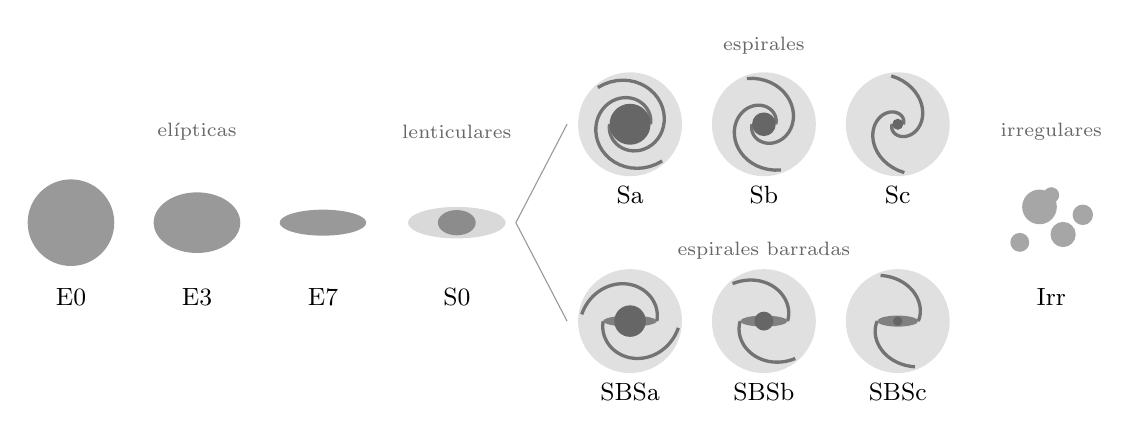
\begin{tikzpicture}[font=\small]
\def\spiralgal#1#2#3#4#5{% x, y, bulge radius, winding rate, bar half-length
  \begin{scope}[shift={(#1,#2)}]
    \fill[black!12] (0,0) circle (0.66);
    \pgfmathsetmacro{\rs}{max(#3,#5)}
    \pgfmathsetmacro{\th}{ln(0.62/\rs)/#4}
    \foreach \a in {0,180}
      \draw[line width=1.2pt, black!55, rotate=\a]
        plot[domain=0:\th, samples=40] ({\rs*exp(#4*\x)*cos(\x r)}, {\rs*exp(#4*\x)*sin(\x r)});
    \ifdim #5pt>0pt \fill[black!50] (0,0) ellipse (#5 and 0.07); \fi
    \fill[black!60] (0,0) circle (#3);
  \end{scope}}
\fill[black!40] (0,0) circle (0.55);
\fill[black!40] (1.6,0) ellipse (0.55 and 0.385);
\fill[black!40] (3.2,0) ellipse (0.55 and 0.165);
\fill[black!15] (4.9,0) ellipse (0.62 and 0.20);
\fill[black!45] (4.9,0) ellipse (0.24 and 0.16);
\draw[black!40] (5.65,0) -- (6.3,1.25);
\draw[black!40] (5.65,0) -- (6.3,-1.25);
\spiralgal{7.1}{1.25}{0.26}{0.16}{0}
\spiralgal{8.8}{1.25}{0.15}{0.28}{0}
\spiralgal{10.5}{1.25}{0.07}{0.45}{0}
\spiralgal{7.1}{-1.25}{0.20}{0.20}{0.34}
\spiralgal{8.8}{-1.25}{0.12}{0.32}{0.30}
\spiralgal{10.5}{-1.25}{0.06}{0.45}{0.26}
\foreach \p/\r in {(12.3,0.2)/0.22,(12.6,-0.15)/0.16,(12.05,-0.25)/0.12,(12.45,0.35)/0.1,(12.85,0.1)/0.13}
  \fill[black!35] \p circle (\r);
\foreach \x/\t in {0/E0,1.6/E3,3.2/E7,4.9/S0}
  \node at (\x,-0.95) {\t};
\foreach \x/\t in {7.1/Sa,8.8/Sb,10.5/Sc}
  { \node at (\x,0.35) {\t}; \node at (\x,-2.15) {SB\t}; }
\node at (12.45,-0.95) {Irr};
\node[font=\scriptsize, black!60] at (1.6,1.15) {elípticas};
\node[font=\scriptsize, black!60] at (4.9,1.15) {lenticulares};
\node[font=\scriptsize, black!60] at (8.8,2.25) {espirales};
\node[font=\scriptsize, black!60] at (8.8,-0.35) {espirales barradas};
\node[font=\scriptsize, black!60] at (12.45,1.15) {irregulares};
\end{tikzpicture}
\par\smallskip{\small La \omterm{def:b3:milky-way-galaxies:types}{secuencia de Hubble} dibujada como un diapasón,
de forma esquemática. Las elípticas se designan según su achatamiento aparente;
la horquilla se bifurca en las lenticulares en espirales normales y de barra,
ordenadas desde bulbos grandes y brazos muy enrollados (a) hasta bulbos pequeños y
brazos abiertos (c); las irregulares cierran la secuencia.}\label{fig:b3:milky-way-galaxies:fork}
\end{omfigure}
% ledger: buta11:hubble

Las clases describen formas observadas en el cielo, y una sola designación oculta un
abanico: una elíptica vista según su eje más corto parece redonda, sea cual sea su
achatamiento real, y los límites entre clases vecinas son una
cuestión de criterio. En un catálogo de las galaxias cercanas, la
Galaxia figura como S(B)bc, una espiral entre Sb y Sc con barra; su gran
vecina Andrómeda (M31) es una Sb, la galaxia del Triángulo (M33) una Sc, y
las Nubes de Magallanes Grande y Pequeña son irregulares.
% ledger: buta11:hubble, mcconn12:local-group

\begin{omfigure}
\centering
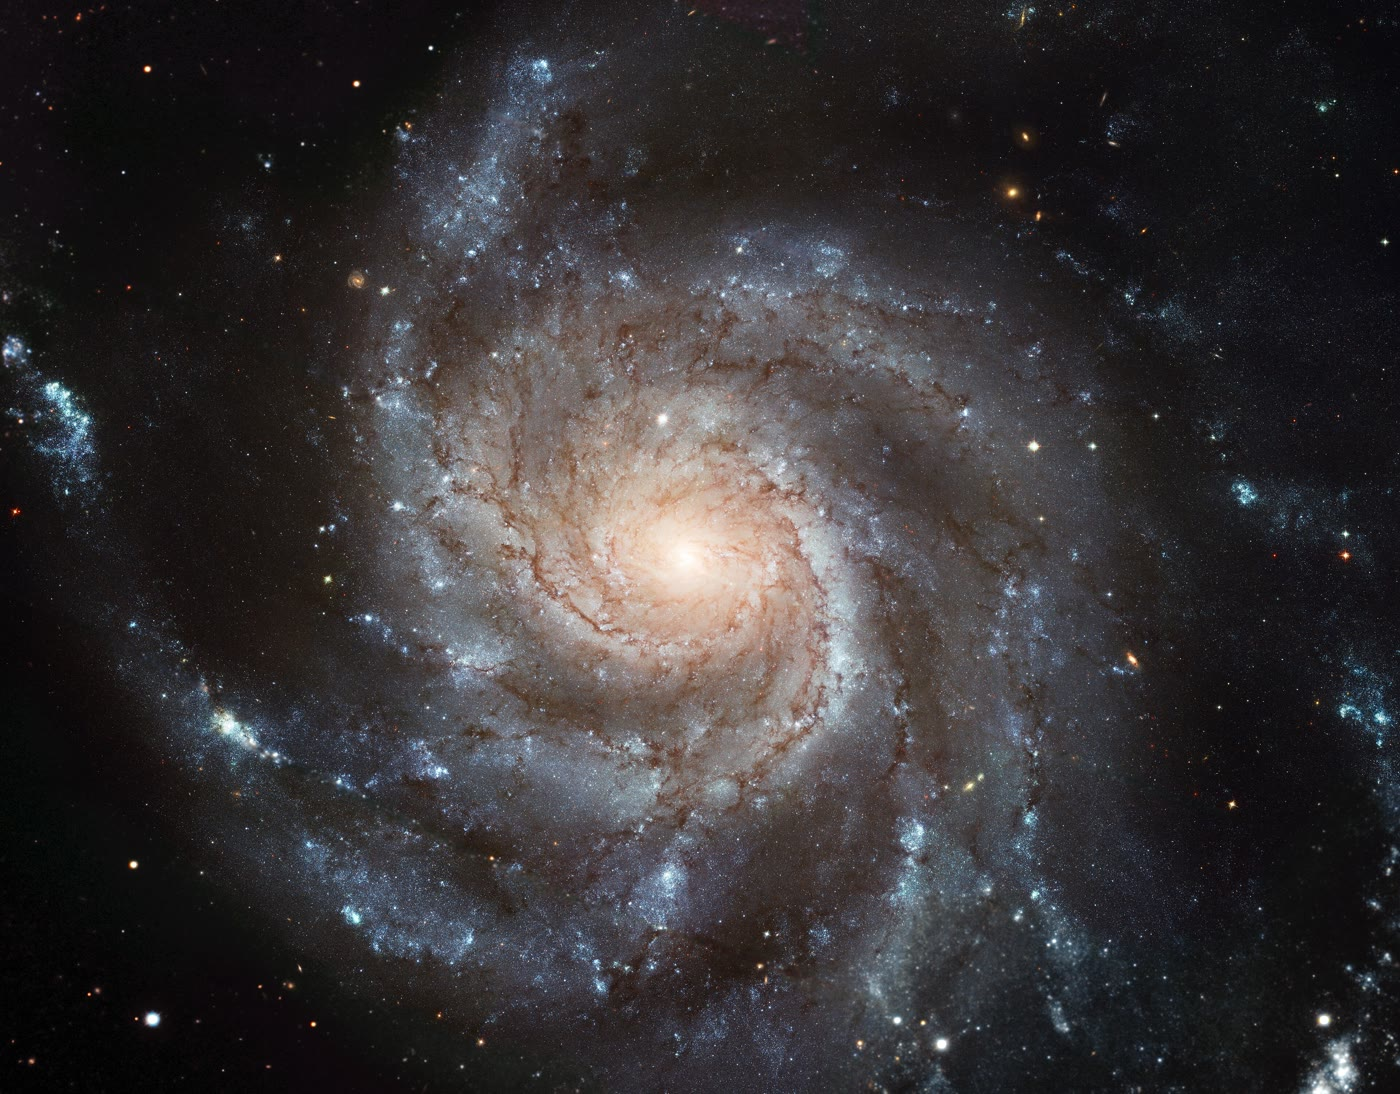
\includegraphics[width=0.66\linewidth]{images/book5/b3-m101.jpg}
\par\smallskip{\small La \omterm{def:b3:milky-way-galaxies:types}{galaxia espiral} M101 vista de frente por el telescopio espacial Hubble,
un mosaico de 51 exposiciones, recortado en sus bordes: un bulbo pequeño,
brillante y amarillento; brazos abiertos, más azulados y salpicados de cúmulos de
estrellas jóvenes; carriles de polvo marrón a lo largo de los brazos. Imagen de ESA y NASA
(Hubble, heic0602), CC BY~4.0.}\label{fig:b3:milky-way-galaxies:m101}
\end{omfigure}
% ledger: photo:b3-m101

¿Por qué no se enrollan los brazos espirales? En un disco cuya \omterm{def:b3:milky-way-galaxies:rotation-curve}{curva de rotación} es plana,
una estrella a la mitad de distancia del centro da una vuelta en la mitad de tiempo.
Una espiral de estrellas se enrollaría más cerrada en cada vuelta, y tras unas pocas vueltas
del disco sería una espiral muy apretada (véase el \cref{exo:b3:milky-way-galaxies:11}).

\begin{definition}[Teoría de las ondas de densidad]\label{def:b3:milky-way-galaxies:density-wave}
La \emph{teoría de las ondas de densidad}\index{teoría de las ondas de densidad} explica los brazos espirales
como una onda de mayor densidad en un disco, un patrón espiral que gira
de forma rígida a su propia velocidad angular, la velocidad del patrón, mientras las estrellas y
el gas se desplazan a través de él, frenándose al entrar en el brazo abarrotado y
acelerándose al salir, como los coches al atravesar un atasco.
\end{definition}

La teoría, propuesta en 1964, libra a los brazos del problema del enrollamiento.
El gas que entra en un brazo se comprime y allí se forman estrellas: los brazos quedan marcados por las estrellas jóvenes
y por el gas luminoso, mientras que las estrellas viejas se reparten de forma mucho más uniforme. Si los brazos son ondas de larga vida
sigue siendo objeto de debate; las simulaciones por ordenador de discos
suelen producir brazos transitorios, que se disuelven y se vuelven a formar,
y una galaxia de paso o una barra pueden impulsar
una espiral de dos brazos.
% ledger: dobbs14:density-wave

\begin{definition}[Agujero negro supermasivo]\label{def:b3:milky-way-galaxies:smbh}
Un \emph{agujero negro supermasivo}\index{agujero negro supermasivo} es un agujero
negro de un millón de masas solares o más en el centro de una galaxia.
\end{definition}

En el centro de la Galaxia, la fuente de radio compacta Sagitario~A* (Sgr~A*)
(Sgr~A*) se encuentra entre estrellas en órbitas cerradas y rápidas. Sus órbitas requieren una
masa central de unos cuatro millones de soles, $\num[separate-uncertainty=true]{4.2 \pm 0.2 e6}$
masas solares en una revisión de las medidas. Sgr~A* apenas se mueve
respecto de las galaxias lejanas: una vez eliminada la órbita del Sol,
su movimiento residual es como máximo de unos pocos kilómetros por segundo, por lo que
retiene al menos una cuarta parte de esa masa. Su tamaño es comparable al de su radio
de Schwarzschild, y su densidad, superior a \num{4e23} masas solares por
parsec cúbico, es muy cercana a la esperada para un agujero negro: la evidencia
de que Sgr~A* es uno es abrumadora.
% ledger: reid20:sgra, bhg16:structure, gravity19:r0

\begin{definition}[Grupo Local; cúmulo de galaxias]\label{def:b3:milky-way-galaxies:groups}
El \emph{Grupo Local}\index{Grupo Local} es el conjunto de galaxias ligadas
gravitacionalmente, dominado por la Vía Láctea y Andrómeda, cada una con
sus galaxias satélite. Un \emph{cúmulo de galaxias}\index{cúmulo de galaxias} es
uno de los sistemas ligados gravitacionalmente más grandes: muchas galaxias retenidas,
con un gas caliente que emite rayos X, en un pozo común formado sobre todo por
materia oscura.
\end{definition}

Más de cien galaxias se encuentran a menos de \qty{3}{Mpc} del Sol, la mayoría
de ellas enanas. La Gran Nube de Magallanes está a unos \qty{50}{kpc}, Andrómeda a
\qty{783}{kpc} y se acerca a nosotros a \qty{300}{km.s^{-1}}, y los miembros
ligados del grupo se hallan a unos \qty{1.06}{Mpc} de su centro de
masas, entre la Galaxia y Andrómeda, donde se apartan de la
expansión del Universo. Su masa, a partir del movimiento de las dos galaxias grandes
una hacia la otra, es del orden de \num{5e12} masas solares. En un
\omterm{def:b3:milky-way-galaxies:groups}{cúmulo masivo de galaxias} el gas caliente, a unos \qty{e8}{K}, tiene alrededor de diez
veces la masa de las estrellas; las galaxias y el gas juntos son demasiado ligeros para
la profundidad del pozo gravitatorio, y la mayor parte de la masa del cúmulo,
del orden de \num{e15} masas solares, es oscura.
% ledger: mcconn12:local-group, kravtsov12:clusters

\section{La escalera de distancias}\label{sec:b3:milky-way-galaxies:ladder}

Un paralaje proporciona una distancia solo por geometría, pero los paralajes disminuyen
con la distancia. El mejor catálogo de ellos mide un paralaje con una
incertidumbre de 0.02 a \qty{0.03}{mas} para estrellas más brillantes que la
magnitud~15, de modo que una distancia con un error del \qty{10}{\percent} llega hasta
unos \qty{4}{kpc}; la Gran Nube de Magallanes, a \qty{50}{kpc}, tiene un
paralaje de \qty{0.02}{mas}. Más allá, las distancias se apoyan en objetos cuya
luminosidad es conocida.
% ledger: gaia:dr3, freedman19:trgb

\begin{definition}[Candela estándar; escalera de distancias]\label{def:b3:milky-way-galaxies:ladder}
Una \emph{candela estándar}\index{candela estándar} es una clase de objetos
cuya magnitud absoluta es conocida, o puede inferirse a partir de una propiedad
medida de forma independiente de la distancia, de modo que su magnitud aparente proporciona
su módulo de distancia. La \emph{escalera de distancias}\index{escalera de distancias} es
la cadena de métodos, cada uno calibrado sobre objetos lo bastante cercanos como para
medirse también con el método anterior, que lleva las distancias desde los
paralajes hasta el Universo en expansión.
\end{definition}

\begin{definition}[Variable cefeida; ley de Leavitt]\label{def:b3:milky-way-galaxies:cepheid}
Una \emph{variable cefeida}\index{variable cefeida} es una estrella joven, luminosa y
pulsante, cuyo brillo varía con un periodo estrictamente regular,
de unos días a varias semanas. La \emph{ley de Leavitt}\index{ley de Leavitt},
o relación periodo--luminosidad, es la relación lineal entre la magnitud absoluta media
de una cefeida y el logaritmo de su periodo; a periodos más largos,
estrellas más brillantes.
\end{definition}

La relación se descubrió en la Pequeña Nube de Magallanes, cuyas estrellas
están todas a casi la misma distancia, en 1908. El polvo de la galaxia que
alberga una cefeida la atenúa y la enrojece; pero la atenuación es mayor
en el visible que en el infrarrojo cercano, en una razón fija para un tipo dado de
polvo, y la combinación $W_I = I - 1.55\,(V - I)$ de las magnitudes en
las bandas I y V, el índice de Wesenheit, se elige de modo que la atenuación
se cancele. La figura siguiente muestra la relación para 2315 cefeidas de la Gran Nube de Magallanes:
la \omterm{def:b3:milky-way-galaxies:cepheid}{ley de Leavitt} es una recta muy ajustada, con una dispersión de
\qty{0.078}{mag}, es decir, un \qty{3.6}{\percent} en distancia para una sola
estrella.
% ledger: sos15:leavitt, data:b5-ogle-lmc-cep

\begin{omfigure}
\centering
\begin{tikzpicture}
\begin{axis}[width=0.80\linewidth, height=0.52\linewidth,
  xmin=-0.05, xmax=1.6, ymin=10, ymax=16.6, y dir=reverse,
  xlabel={$\log_{10}(P/\mathrm{d})$}, ylabel={Índice de Wesenheit $W_I$ (mag)},
  tick label style={font=\scriptsize}, label style={font=\small},
  legend style={font=\scriptsize, at={(0.5,-0.17)}, anchor=north, legend columns=3, draw=none, cells={anchor=west}, /tikz/every even column/.append style={column sep=1em}},
  legend image post style={scale=2.2}]
\addplot[only marks, mark=*, mark size=0.45pt, omDef, opacity=0.6] table[x=logp, y=w] {figdata/out/bachelor-3-distance_ladder-pl.dat};
\addlegendentry{Cefeidas}
\addplot[only marks, mark=x, mark size=1.6pt, red!70!black] table[x=logp, y=w] {figdata/out/bachelor-3-distance_ladder-clipped.dat};
\addlegendentry{apartadas ($>3\sigma$)}
\addplot[thick, black] table[x=logp, y=w_fit] {figdata/out/bachelor-3-distance_ladder-fit.dat};
\addlegendentry{ajuste}
\node[font=\scriptsize, anchor=south west, fill=white, inner sep=1pt] at (axis cs:0.55,11.0) {$W_I = -3.315\log_{10}P + 15.889$};
\end{axis}
\end{tikzpicture}
\par\smallskip{\small La \omterm{def:b3:milky-way-galaxies:cepheid}{ley de Leavitt} en la Gran Nube de Magallanes:
el índice de Wesenheit de 2315 cefeidas que pulsan en su modo fundamental
frente al logaritmo de su periodo (sondeo OGLE, Soszy\'nski y
otros, 2015, a través del CDS). Las estrellas más brillantes están más arriba. Una recta
ajustada por mínimos cuadrados, tras apartar 92 estrellas situadas a más de
tres desviaciones típicas de ella, reproduce la relación publicada
($-3.314$, $15.888$). Con el módulo de distancia de la Nube, 18.477, la recta
proporciona la magnitud absoluta de Wesenheit de cualquier cefeida a partir de su periodo.}\label{fig:b3:milky-way-galaxies:leavitt}
\end{omfigure}
% ledger: data:b5-ogle-lmc-cep, sos15:leavitt, freedman19:trgb

\begin{definition}[Punta de la rama de las gigantes rojas]\label{def:b3:milky-way-galaxies:trgb}
La \emph{punta de la rama de las gigantes rojas}\index{punta de la rama de las gigantes rojas}
(TRGB) es el límite superior nítido de las luminosidades de las gigantes rojas de
una \omterm{def:b3:milky-way-galaxies:populations}{población estelar} antigua, fijado por la ignición del helio en sus núcleos,
el destello de helio; en la banda I se sitúa casi en la misma magnitud absoluta
en toda población antigua, $M_I \approx -4.05$ con un color
$V - I = 1.6$, y depende solo débilmente de la composición química.
\end{definition}

La punta se mide en los halos dispersos de las galaxias, donde hay
poco polvo y poca aglomeración; utiliza estrellas viejas del halo donde las cefeidas usan
estrellas jóvenes del disco, y los dos métodos no comparten ninguna física. Las cefeidas y la
TRGB alcanzan unas decenas de megapársecs, hacia galaxias donde una \omterm{def:b3:milky-way-galaxies:ladder}{candela estándar} rara y mucho más
brillante ha estallado: una supernova de tipo~Ia, la
explosión termonuclear de una enana blanca, recordada de los libros de física,
cuya magnitud absoluta en el máximo, una vez corregida por la
forma de su curva de luz y de su color, es
$M_B = \qty[separate-uncertainty=true]{-19.253 \pm 0.027}{mag}$. Tales
supernovas se observan a lo largo de cientos de megapársecs.
% ledger: freedman19:trgb, riess22:h0

\begin{definition}[Relación de Tully--Fisher]\label{def:b3:milky-way-galaxies:tully-fisher}
La \emph{relación de Tully--Fisher}\index{relación de Tully--Fisher} es la
correlación entre la luminosidad, o mejor la masa de estrellas y de gas,
de una \omterm{def:b3:milky-way-galaxies:types}{galaxia espiral} y la velocidad de su \omterm{def:b3:milky-way-galaxies:rotation-curve}{curva de rotación} plana; en su
forma bariónica, $M_\mathrm{b} = A\,V^4$, se cumple desde unos 30 hasta
\qty{300}{km.s^{-1}}.
\end{definition}

El espectro de 21~cm de una galaxia proporciona su velocidad máxima de rotación, y la
relación da su luminosidad, con independencia de su distancia, y su flujo
permite entonces fijar la distancia: un peldaño para \omterm{def:b3:milky-way-galaxies:types}{galaxias espirales} demasiado lejanas para
estrellas individuales. La Galaxia, por su luminosidad y su rotación, se ajusta a la relación.
% ledger: mcgaugh00:btf, nrao:hi-line, bhg16:structure

\begin{omfigure}
\centering
\pgfplotstableread{figdata/out/bachelor-3-distance_ladder-ladder.dat}\laddertab
\pgfplotstableread{figdata/out/bachelor-3-distance_ladder-anchors.dat}\anchortab
\pgfplotstablegetelem{0}{d_hi}\of{\laddertab}\let\plxhi\pgfplotsretval
\pgfplotstablegetelem{1}{d_lo}\of{\laddertab}\let\cephlo\pgfplotsretval
\pgfplotstablegetelem{1}{d_hi}\of{\laddertab}\let\cephhi\pgfplotsretval
\pgfplotstablegetelem{3}{d_lo}\of{\laddertab}\let\snlo\pgfplotsretval
\pgfplotstablegetelem{3}{d_hi}\of{\laddertab}\let\snhi\pgfplotsretval
\pgfplotstablegetelem{1}{d}\of{\anchortab}\let\mthirtyone\pgfplotsretval
\pgfplotstablegetelem{2}{d}\of{\anchortab}\let\nfourtwo\pgfplotsretval
\begin{tikzpicture}
\begin{axis}[width=0.92\linewidth, height=0.42\linewidth,
  xmode=log, xmin=1e-3, xmax=2e6, ymin=0.4, ymax=4.9,
  ytick={1,2,3,4}, yticklabels={paralajes, cefeidas, TRGB, SNe~Ia},
  xtick={1e-3,1e-2,1e-1,1,10,100,1e3,1e4,1e5,1e6},
  xticklabels={1\,pc,,,1\,kpc,,,1\,Mpc,,,1\,Gpc},
  xlabel={distancia}, tick label style={font=\scriptsize}, label style={font=\small},
  y tick label style={font=\small}, axis y line*=left, axis x line*=bottom]
\draw[line width=7pt, omDef!70] (axis cs:1e-3,1) -- (axis cs:\plxhi,1);
\draw[line width=7pt, omMeth!70] (axis cs:\cephlo,2) -- (axis cs:\cephhi,2);
\draw[line width=7pt, omProp!70] (axis cs:\cephlo,3) -- (axis cs:\cephhi,3);
\draw[line width=7pt, red!60] (axis cs:\snlo,4) -- (axis cs:\snhi,4);
\draw[densely dotted, thick] (axis cs:\cephlo,0.4) -- (axis cs:\cephlo,4.55) node[anchor=south, font=\scriptsize] {LMC};
\draw[densely dotted, thick] (axis cs:\mthirtyone,0.4) -- (axis cs:\mthirtyone,4.55) node[anchor=south, font=\scriptsize] {M31};
\draw[densely dotted, thick] (axis cs:\nfourtwo,0.4) -- (axis cs:\nfourtwo,4.55) node[anchor=south, font=\scriptsize] {NGC~4258};
\draw[->, thick, black!60] (axis cs:\plxhi,1.25) to[out=30, in=200] (axis cs:\cephlo,1.75);
\draw[->, thick, black!60] (axis cs:\cephhi,2.25) to[out=40, in=220] (axis cs:\snlo,3.75);
\end{axis}
\end{tikzpicture}
\par\smallskip{\small Los peldaños de la \omterm{def:b3:milky-way-galaxies:ladder}{escalera de distancias}, con las
distancias en las que se emplea cada uno aquí: paralajes del mejor catálogo,
con un error de \qty{10}{\percent} hasta \qty{4}{kpc}; las cefeidas y la TRGB desde la
Gran Nube de Magallanes a las galaxias anfitrionas de las supernovas de tipo~Ia más cercanas,
hasta \qty{45}{Mpc}; las supernovas de la expansión suave, con corrimientos al rojo entre
0.023 y 0.15 (\qtyrange{96}{616}{Mpc} para $H_0 = 73$). En punteado: dos anclajes de
la escala de las cefeidas con distancias geométricas (binarias eclipsantes en la
LMC, máseres de agua que orbitan el agujero negro de NGC~4258), y M31, la
espiral grande más cercana. Flechas: cada peldaño se calibra con objetos que el
peldaño inferior también mide, las cefeidas de la Galaxia mediante sus paralajes,
las supernovas de galaxias cercanas mediante las cefeidas y la TRGB de sus
anfitrionas.}\label{fig:b3:milky-way-galaxies:ladder-rungs}
\end{omfigure}
% ledger: gaia:dr3, riess22:h0, freedman19:trgb, mcconn12:local-group

En lo alto de la escalera, las supernovas miden la expansión del
Universo. La ley de Hubble, recordada de los libros de física, hace que la
velocidad de recesión $cz$ de una galaxia lejana sea proporcional a su distancia $d$,
$cz = H_0 d$ para corrimientos al rojo pequeños $z$; la constante de Hubble $H_0$ es la
pendiente, y las supernovas, con sus distancias obtenidas de la escalera, la proporcionan.

\begin{definition}[Tensión de Hubble]\label{def:b3:milky-way-galaxies:tension}
La \emph{tensión de Hubble}\index{tensión de Hubble} es la discrepancia
entre el valor de la constante de Hubble medido localmente con la
\omterm{def:b3:milky-way-galaxies:ladder}{escalera de distancias} y el valor inferido a partir del fondo cósmico de
microondas con el modelo cosmológico estándar.
\end{definition}

\begin{dated}{2022}
Las cefeidas de las galaxias anfitrionas de 42 supernovas de tipo~Ia, ancladas en
las paralajes de Gaia, los máseres de NGC~4258 y las binarias eclipsantes de la
Gran Nube de Magallanes, dan
$H_0 = \qty[separate-uncertainty=true]{73.04 \pm 1.04}{km.s^{-1}.Mpc^{-1}}$.
La \omterm{def:b3:milky-way-galaxies:trgb}{punta de la rama de las gigantes rojas}, al calibrar unas cien supernovas,
dio en 2019 $H_0 = 69.8 \pm 0.8 \pm \qty{1.7}{km.s^{-1}.Mpc^{-1}}$
(estadística y sistemática). El mapa del fondo cósmico de
microondas del satélite Planck, interpretado con el modelo cosmológico estándar, implica
$H_0 = \qty[separate-uncertainty=true]{67.4 \pm 0.5}{km.s^{-1}.Mpc^{-1}}$.
El valor de las cefeidas y el del fondo difieren en cinco desviaciones
típicas; el valor de la TRGB queda entre ambos. El origen de la
discrepancia no se conoce: un error aún no hallado en una de las escaleras,
o física que falta en el modelo.
\end{dated}
% ledger: riess22:h0, freedman19:trgb, planck18:h0

\begin{inthelab}[Un satélite astrométrico y su catálogo]
El satélite Gaia barre el cielo siguiendo un patrón programado, de modo que cada
estrella se mide una y otra vez a lo largo de la misión. En tierra, las
unidades de coordinación de un consorcio de procesamiento de datos convierten estas
mediciones en una posición, un paralaje y un movimiento propio para cada una de
más de mil millones de fuentes: de los pequeños desplazamientos de una estrella en el cielo,
el paralaje es la parte que se repite cada año y el movimiento propio
es la parte que se acumula. Cada catálogo se publica junto con artículos que
describen su procesamiento y su validación, y toda distancia de las
figuras de esta sección que se apoya en un paralaje se apoya en un
catálogo de este tipo.
\end{inthelab}

\begin{dated}{2022}
El tercer catálogo de Gaia, publicado el 13 de junio de 2022 con datos de 34 meses de
observaciones, ofrece posiciones, paralajes y movimientos propios para unas
1.46~mil millones de fuentes, de magnitud~3 a~21, y velocidades radiales medias
para 33~millones de estrellas. Sus incertidumbres de paralaje son de 0.02 a
\qty{0.03}{mas} para estrellas más brillantes que la magnitud~15, \qty{0.07}{mas} en
la magnitud~17, y \qty{0.5}{mas} en la magnitud~20.
\end{dated}
% ledger: gaia:dr3

\section{Ejercicios}

\begin{exercise}[$\star$]\label{exo:b3:milky-way-galaxies:1}
El año galáctico del Sol. (a)~Con $R_0 = \qty{8.178}{kpc}$ y
$V_0 = \qty{229}{km.s^{-1}}$, calcúlese el periodo de la órbita del Sol alrededor del
centro galáctico, en millones de años. (b)~¿Cuántas vueltas ha dado el Sol
desde que se formó el Sistema Solar, hace \qty{4.54}{Gyr}?
\end{exercise}

\begin{exercise}[$\star$]\label{exo:b3:milky-way-galaxies:2}
El movimiento reflejo de Sgr~A*. (a)~Un movimiento propio de \qty{1}{mas} al año
a \qty{1}{kpc} equivale a una velocidad transversal de \qty{1}{au} al año: exprésese en
kilómetros por segundo. (b)~Sgr~A*, supuesto en reposo en el centro galáctico
a \qty{8.178}{kpc}, se desplaza a lo largo del plano galáctico \qty{6.411}{mas}
al año. Calcúlese la velocidad del Sol alrededor del centro y compárese con el
valor de referencia, \qty[separate-uncertainty=true]{248 \pm 3}{km.s^{-1}}. (c)~Réstese el
movimiento peculiar del Sol en la dirección de rotación, \qty{11}{km.s^{-1}}, y
compárese con $V_0$ de la \omterm{def:b3:milky-way-galaxies:rotation-curve}{curva de rotación}.
\end{exercise}

\begin{exercise}[$\star$]\label{exo:b3:milky-way-galaxies:3}
Clasificación de las elípticas. (a)~Las isofotas de una \omterm{def:b3:milky-way-galaxies:types}{galaxia elíptica} tienen una
razón de ejes de 0.6: indíquese su clase. (b)~¿Qué razón de ejes tiene una E7?
(c)~¿Por qué una galaxia E0 puede ser un sistema achatado?
\end{exercise}

\begin{exercise}[$\star$]\label{exo:b3:milky-way-galaxies:4}
Anclas. Calcúlense las distancias de la Gran Nube de Magallanes
($\mu = 18.477$), Andrómeda ($\mu = 24.47$) y NGC~4258
($\mu = 29.398$). ¿Qué paralaje tendría una estrella de la Nube, y por qué
no puede medirse la distancia de la Nube mediante paralajes?
\end{exercise}

\begin{exercise}[$\star\star$]\label{exo:b3:milky-way-galaxies:5}
A partir de las \omterm{def:b3:milky-way-galaxies:rotation-curve}{constantes de Oort} $A = \qty{15.3}{km.s^{-1}.kpc^{-1}}$ y
$B = \qty{-11.9}{km.s^{-1}.kpc^{-1}}$: (a)~calcúlese la velocidad angular del
\omterm{def:b3:milky-way-galaxies:lsr}{estándar local de reposo} y, con $R_0 = \qty{8.178}{kpc}$, la velocidad circular $V_0$;
(b)~calcúlese la pendiente de la \omterm{def:b3:milky-way-galaxies:rotation-curve}{curva de rotación} en el Sol. (c)~Compárese
con la \omterm{def:b3:milky-way-galaxies:rotation-curve}{curva de rotación} de las gigantes rojas ($V_0 = \qty{229.0}{km.s^{-1}}$,
pendiente \qty{-1.7}{km.s^{-1}} por kiloparsec) y sugiérase por qué las dos
difieren, dado que la misma medición halló $C$ y $K$ distintos de cero.
\end{exercise}

\begin{exercise}[$\star\star$]\label{exo:b3:milky-way-galaxies:6}
Una \omterm{def:b3:milky-way-galaxies:rotation-curve}{curva de rotación} plana y la densidad local. (a)~Para una galaxia esférica
con \omterm{def:b3:milky-way-galaxies:rotation-curve}{curva de rotación} plana a \qty{229}{km.s^{-1}}, calcúlese la densidad a
\qty{8.178}{kpc}, en masas solares por parsec cúbico
($G = \qty{4.301e-6}{kpc.(km.s^{-1})^2}$ por masa solar). (b)~Demuéstrese que
una masa solar por parsec cúbico equivale a \qty{37.96}{GeV.cm^{-3}}, y exprésese
la densidad local de materia oscura, \qty{0.30}{GeV.cm^{-3}}, en masas solares
por parsec cúbico. (c)~¿Por qué es mayor la densidad de (a)?
\end{exercise}

\begin{exercise}[$\star\star$]\label{exo:b3:milky-way-galaxies:7}
Distancia de una cefeida. En una \omterm{def:b3:milky-way-galaxies:types}{galaxia espiral} ficticia, una cefeida de periodo
\qty{30}{d} tiene un índice de Wesenheit medio $W_I = \qty{25.00}{mag}$.
(a)~Usando la \omterm{def:b3:milky-way-galaxies:cepheid}{ley de Leavitt} de la Gran Nube de Magallanes,
$W_I = -3.314\log_{10}P + 15.888$, y el módulo de distancia de la Nube
18.477, calcúlese la magnitud absoluta de Wesenheit de la cefeida. (b)~Calcúlese
la distancia de la galaxia. (c)~La dispersión de la ley es \qty{0.077}{mag}: ¿cuál es
el error relativo de distancia a partir de una cefeida, y a partir de cincuenta?
\end{exercise}

\begin{exercise}[$\star\star$]\label{exo:b3:milky-way-galaxies:8}
Distancia TRGB. En el halo de una galaxia ficticia, la \omterm{def:b3:milky-way-galaxies:trgb}{punta de la rama de las gigantes rojas}
se encuentra en $I = \qty{26.00}{mag}$; el polvo a lo largo de la línea de
visión atenúa la banda I en \qty{0.05}{mag}. Con $M_I = -4.05$, calcúlese el
módulo de distancia y la distancia. ¿Qué significa una incertidumbre de
\qty{0.04}{mag} en la punta, en distancia?
\end{exercise}

\begin{exercise}[$\star\star$]\label{exo:b3:milky-way-galaxies:9}
La constante de Hubble a partir de supernovas. Para una supernova de la expansión suave,
$\log_{10}(cz) - 0.2\,m_B = a_B$, la ordenada en el origen del
diagrama de Hubble de las supernovas, y el módulo de distancia es
$m_B - M_B = 5\log_{10}(d/\mathrm{Mpc}) + 25$. (a)~Demuéstrese que
$\log_{10}H_0 = 0.2\,M_B + a_B + 5$ ($H_0$ en kilómetros por segundo por
megaparsec). (b)~Con $M_B = -19.253$ y $a_B = 0.714158$, calcúlese $H_0$.
(c)~¿Qué $M_B$ daría $H_0 = \qty{67.4}{km.s^{-1}.Mpc^{-1}}$? ¿En cuántas
magnitudes, y en qué fracción de las distancias, difieren las dos
calibraciones?
\end{exercise}

\begin{exercise}[$\star\star\star$]\label{exo:b3:milky-way-galaxies:10}
De dónde procede la ley de Tully--Fisher. (a)~Una galaxia de disco de masa $M$
y radio $R$ gira a $V$: demuéstrese que $M \approx RV^2/G$. (b)~Si todas
las \omterm{def:b3:milky-way-galaxies:types}{galaxias espirales} tuvieran la misma densidad superficial media $\Sigma = M/(\pi R^2)$,
demuéstrese que $M \propto V^4$. (c)~Dos galaxias ficticias sobre la misma relación bariónica
giran a 100 y \qty{229}{km.s^{-1}}: ¿cuál es la razón de
sus masas? (d)~Dos galaxias giran a la misma velocidad y tienen la misma
luminosidad; una da cuatro veces el flujo de la otra. Compárense sus
distancias.
\end{exercise}

\begin{exercise}[$\star\star\star$]\label{exo:b3:milky-way-galaxies:11}
El problema del enrollamiento. Un disco gira con una curva plana a
\qty{229}{km.s^{-1}}. (a)~Conviértase esta velocidad a kiloparsecs por mil millones de
años. (b)~Un brazo recto de estrellas se extiende en el instante inicial desde 4 hasta
\qty{12}{kpc}. Calcúlense los periodos orbitales en ambos extremos. (c)~Transcurridos
\qty{1}{Gyr}, ¿en qué ángulo se ha adelantado su extremo interior respecto del exterior?
¿Cuántas vueltas de espiral representa eso y qué aspecto tendría el
brazo? (d)~¿Cómo evita una onda de densidad este problema?
\end{exercise}

\begin{exercise}[$\star\star\star$]\label{exo:b3:milky-way-galaxies:12}
El agujero negro del centro. Tómese la masa central igual a
\num{4.2e6} masas solares y $R_0 = \qty{8178}{pc}$. (a)~La estrella S2
orbita en torno a él en \num{16}~años: calcúlese el semieje mayor de su órbita en
unidades astronómicas (tercera ley de Kepler en unidades solares, $a^3 = MP^2$ con
$a$ en ua, $P$ en años y $M$ en masas solares) y su tamaño angular visto
desde la Tierra. (b)~Calcúlese el radio de Schwarzschild del agujero negro en
metros y en unidades astronómicas, y el ángulo que su diámetro
subtiende desde la Tierra, en microsegundos de arco. (c)~Calcúlese la densidad media
de la masa contenida en su radio de Schwarzschild, en masas solares por
parsec cúbico, y compárese con la cota inferior fijada por el movimiento de Sgr~A*,
\num{4e23} masas solares por parsec cúbico.
\end{exercise}

\section{Problema: pesando la Galaxia}

\begin{problem}[{Problema de fin de semana --- a partir de los movimientos de estrellas y gas hasta
la materia oscura dentro de \qty{20}{kpc}}]
\label{pb:b3:milky-way-galaxies:1}
Tómese $R_0 = \qty{8.18}{kpc}$, $G = \qty{4.301e-6}{kpc.(km.s^{-1})^2}$ por
masa solar, y \qty{4.74}{km.s^{-1}} para un movimiento propio de
\qty{1}{mas} al año a \qty{1}{kpc}. Todas las velocidades son relativas al
LSR. Úsense los teoremas de Oort y del punto tangente del capítulo, y la
aproximación esférica $M = RV^2/G$ para las masas dinámicas.

\medskip\noindent\textbf{Parte I --- La rotación local.} Un sondeo inventado
de estrellas del nudo rojo, todas a $d = \qty{1.00}{kpc}$ en el plano galáctico,
da una velocidad radial media de \qty{+15.4}{km.s^{-1}} en
$\ell = \ang{45}$ y \qty{-15.2}{km.s^{-1}} en $\ell = \ang{135}$, y
movimientos propios medios en longitud de \qty{-5.91}{mas} al año en
$\ell = \ang{90}$ y \qty{+0.55}{mas} al año en $\ell = \ang{0}$.
\begin{enumerate}
\item ¿Qué predice la fórmula de Oort para las velocidades radiales en
  $\ell = \ang{45}$, \ang{90}, \ang{135} y \ang{180}?
\item Calcúlese $A$ a partir de las dos velocidades radiales.
\item Calcúlese $B$ a partir del movimiento propio en $\ell = \ang{90}$.
\item Calcúlese de nuevo $B$ a partir del movimiento propio en $\ell = \ang{0}$, y
  compárese.
\item Calcúlense la velocidad angular del LSR y la velocidad circular
  $V_0$.
\item Calcúlese la pendiente de la \omterm{def:b3:milky-way-galaxies:rotation-curve}{curva de rotación} en el Sol. ¿Es la curva
  creciente, plana o decreciente?
\item Calcúlese el periodo de la órbita del Sol y el número de vueltas en
  \qty{4.54}{Gyr}.
\end{enumerate}

\medskip\noindent\textbf{Parte II --- La curva de rotación interior.} Tómese
$V_0 = \qty{229}{km.s^{-1}}$. Las velocidades radiales más altas en los
perfiles de 21 cm en $\ell = \ang{40}$, \ang{50}, \ang{60} y \ang{70} son
82.9, 55.6, 32.4 y \qty{14.9}{km.s^{-1}}.
\begin{enumerate}[resume]
\item ¿Por qué el método del punto tangente necesita $\ang{0} < \ell < \ang{90}$
  (o el cuadrante simétrico), y ¿por qué falla más allá del círculo solar?
\item Calcúlese el radio del punto tangente para cada longitud.
\item Calcúlese $V(R)$ en cada punto tangente.
\item ¿En cuánto, en kilohercios, se desplaza la línea del gas en el punto tangente
  en $\ell = \ang{40}$ respecto de su frecuencia en reposo,
  \qty{1420.405751}{MHz}, y en qué sentido?
\item Compárese con la curva de las gigantes rojas, que da \qty{226.8}{km.s^{-1}}
  a \qty{5.27}{kpc} y \qty{229.6}{km.s^{-1}} a \qty{7.22}{kpc}. ¿Es la
  curva interior creciente, plana o decreciente?
\item Si la velocidad en el punto tangente en $\ell = \ang{40}$ fuera la de
  una masa puntual en el centro que lleva al Sol a $V_0$, ¿cuál sería?
  ¿Qué dice la comparación sobre la distribución de la masa?
\end{enumerate}

\medskip\noindent\textbf{Parte III --- La masa visible.} Úsese el modelo de masas
del capítulo, en unidades de masas solares y kiloparsecs: un
bulbo de Plummer $M = \num{1.067e10}$, $b = 0.3$; un disco fino de Miyamoto--Nagai
$M = \num{3.944e10}$, $a = 5.3$, $b = 0.25$; un \omterm{def:b3:milky-way-galaxies:structure}{disco grueso} de la misma
masa con $a = 2.6$, $b = 0.8$.
\begin{enumerate}[resume]
\item Calcúlese la masa visible total del modelo y compárese con el
  valor de revisión de la masa estelar de la Galaxia, \qty[separate-uncertainty=true]{5 \pm 1 e10}{} masas
  solares.
\item Calcúlese la velocidad circular del bulbo solo a \qty{20}{kpc}.
\item Calcúlense las del disco fino y las del \omterm{def:b3:milky-way-galaxies:structure}{disco grueso} a \qty{20}{kpc}.
\item Calcúlese la velocidad circular de toda la masa visible a
  \qty{20}{kpc}.
\item Calcúlese lo mismo en $R_0$, y compárese con $V_0$.
\item Si toda la masa visible estuviera concentrada en el centro, ¿cuál sería
  la velocidad a \qty{20}{kpc}? ¿Por qué el valor del modelo se aproxima a ella?
\end{enumerate}

\medskip\noindent\textbf{Parte IV --- La materia oscura.} Las gigantes rojas
dan una velocidad circular de \qty{200}{km.s^{-1}} a \qty{20}{kpc}.
\begin{enumerate}[resume]
\item Calcúlese la masa dinámica dentro de \qty{20}{kpc}.
\item Calcúlese la masa dinámica de la materia visible dentro de
  \qty{20}{kpc}.
\item Calcúlese la masa de materia oscura dentro de \qty{20}{kpc}, y demuéstrese que
  su fracción es $1 - (V_\mathrm{vis}/V)^2$.
\item El halo NFW ajustado a toda la curva tiene
  $\rho_0 = \num{1.06e7}$ masas solares por kiloparsec cúbico y
  $R_s = \qty{14.8}{kpc}$. Calcúlese su masa dentro de \qty{20}{kpc} y la
  fracción oscura que implica. ¿Por qué difiere de la respuesta anterior?
\item Calcúlese la densidad de ese halo en $R_0$, en masas solares por
  parsec cúbico y en \unit{GeV.cm^{-3}} (una masa solar por parsec cúbico
  equivale a \qty{37.96}{GeV.cm^{-3}}).
\item Indíquese la fracción de materia oscura de la masa dentro de \qty{20}{kpc}
  obtenida a partir de la velocidad medida, en por ciento, con dos cifras
  significativas.
\end{enumerate}
\end{problem}
% ledger: gravity19:r0, eilers19:table1, pouliasis17:model1, eilers19:halo, bhg16:structure, nrao:hi-line, const:G, const:au, iau:parsec, usgs:age-earth
